% Chris's Entropy Library - User Guide - Entropy
% Written by Christopher Thomas.

\chapter{Entropy}
\label{sect-entropy}

\section{Shannon Entropy}
\label{sect-entropy-shannon}

\textbf{Entropy} can be thought of as measuring the information content of
a stream of data samples. It is defined (per Shannon 1949) as the amount of
``surprise'' associated with each sample when that sample is considered to
be a discrete symbol drawn from a set of possible symbols with some
probability distribution. The entropy associated with one symbol is given
in Equation \ref{eq-shannon-symbol}, and the average entropy per symbol
associated with a symbol stream is given in Equation
\ref{eq-shannon-stream}. It can be seen from Equation \ref{eq-shannon-symbol}
that symbols with lower probability result in more ``surprise'': rare symbols
are more informative than commonly-seen symbols.

\begin{equation}
H(x_k) = \log_2 \left [ \frac{1}{P(x_k)} \right ] = - \log_2 [ P(x_k) ]
\label{eq-shannon-symbol}
\end{equation}

\begin{equation}
H(X) = - \sum_k P(x_k) \log_2 [ P(x_k) ]
\label{eq-shannon-stream}
\end{equation}

For discrete-valued data, or data such as text that is readily interpreted
as symbols, entropy may be calculated on the raw data values. A histogram
of observed symbols is made, and this is used as the probability
distribution. For continuous-valued data, histogram bins are typically
defined and the bin labels are interpreted as symbols. For data consisting
of event arrival times, time bins are typically defined and the number of
events within each bin are counted. These counts may be taken as individual
symbols or several adjacent time bins may be considered to form a word,
which is used as a symbol for entropy calculations. These approaches are
discussed in more detail in Section \ref{sect-howto}.

% FIXME - Force a page break.
\clearpage
%
\section{Conditional Entropy}
\label{sect-entropy-cond}

\textbf{Conditional entropy} can be thought of as the amount of additional
information learned from samples of variable Y when we already know the
value of a related variable X. This is illustrated in Figure
\ref{fig-cond-def} (left). It is defined by Equation \ref{eq-cond-def}:

\begin{equation}
H(Y|X) = - \sum_{j,k} P(x_j,y_k) \log_2 \left [
\frac{P(x_j,y_k)}{P(x_j)} \right ]
\label{eq-cond-def}
\end{equation}

For the case of independent variables where $P(x_j,y_k) = P(x_j) P(y_k)$,
this reduces to Shannon entropy.

This is generalized to several X variables per Equation \ref{eq-cond-multi};
this case is illustrated in Figure \ref{fig-cond-def} (right).

\begin{equation}
H(Y|X_A,X_B) = - \sum_{j,k,m} P(x_{aj},x_{bk},y_m) \log_2 \left [
\frac{P(x_{aj},x_{bk},y_m)}{P(x_{aj},x_{bk})} \right ]
\label{eq-cond-multi}
\end{equation}

\figdef{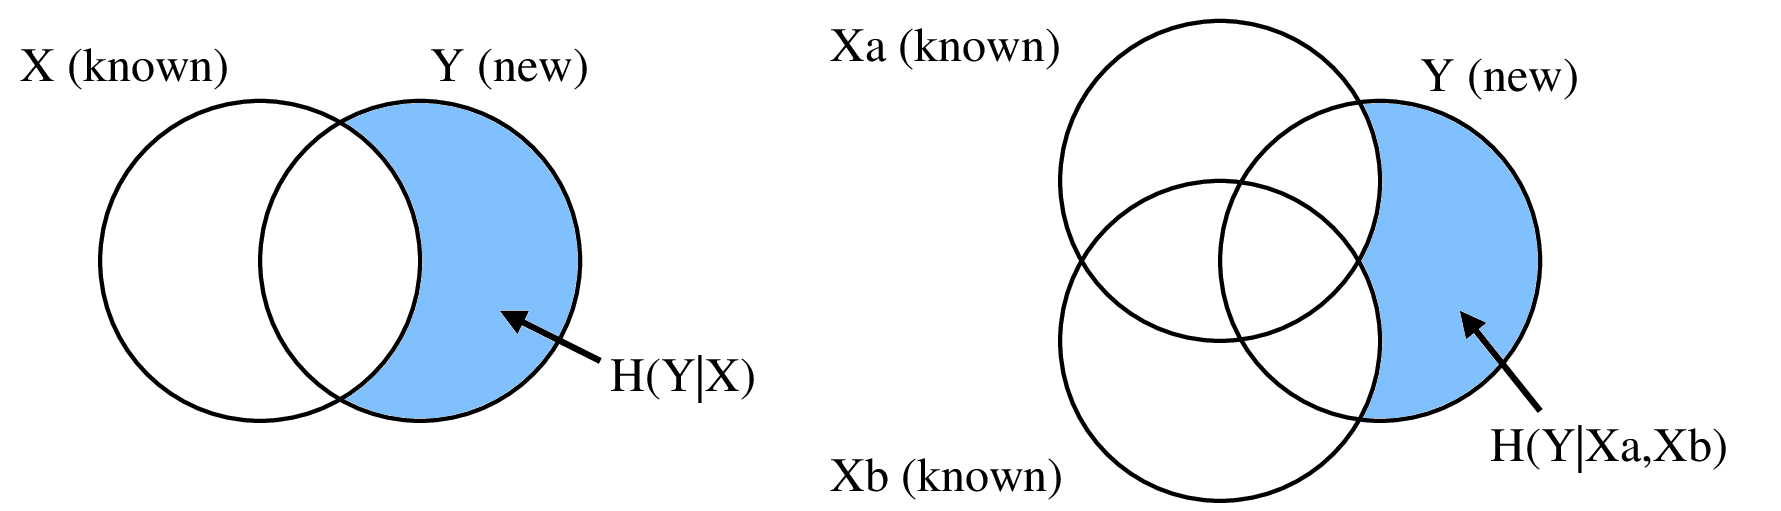
\includegraphics[height=1.5in]
{figs/conditional-entropy-edited.png}}
{Conditional entropy with two signals (left) and three signals (right).}
{fig-cond-def}

% FIXME - Force a page break.
\clearpage
%
\section{Mutual Information}
\label{sect-entropy-mutual}

\textbf{Mutual information} can be thought of as the amount of information
shared between related variables X and Y. Sampling either variable X
\textit{or} variable Y reveals the shared information. This is illustrated
in Figure \ref{fig-mutual-def} (left). Mutual information is defined by
Equation \ref{eq-mutual-def}:

\begin{equation}
I(X,Y) = \sum_{j,k} P(x_j,y_k) \log_2 \left [
\frac{P(x_j,y_k)}{P(x_j) P(y_k)} \right ]
\label{eq-mutual-def}
\end{equation}

For the case of independent variables where $P(x_j,y_k) = P(x_j) P(y_k)$,
this is equal to zero (due to the $log_2(1)$ term).

This is generalized to more than two variables per Equation
\ref{eq-mutual-multi}; this case is illustrated in Figure
\ref{fig-mutual-def} (right).

\begin{equation}
I(X,Y,Z) = \sum_{j,k,m} P(x_j,y_k,z_m) \log_2 \left [
\frac{P(x_j,y_k,z_m)}{P(x_j) P(y_k) P(z_m)} \right ]
\label{eq-mutual-multi}
\end{equation}

\figdef{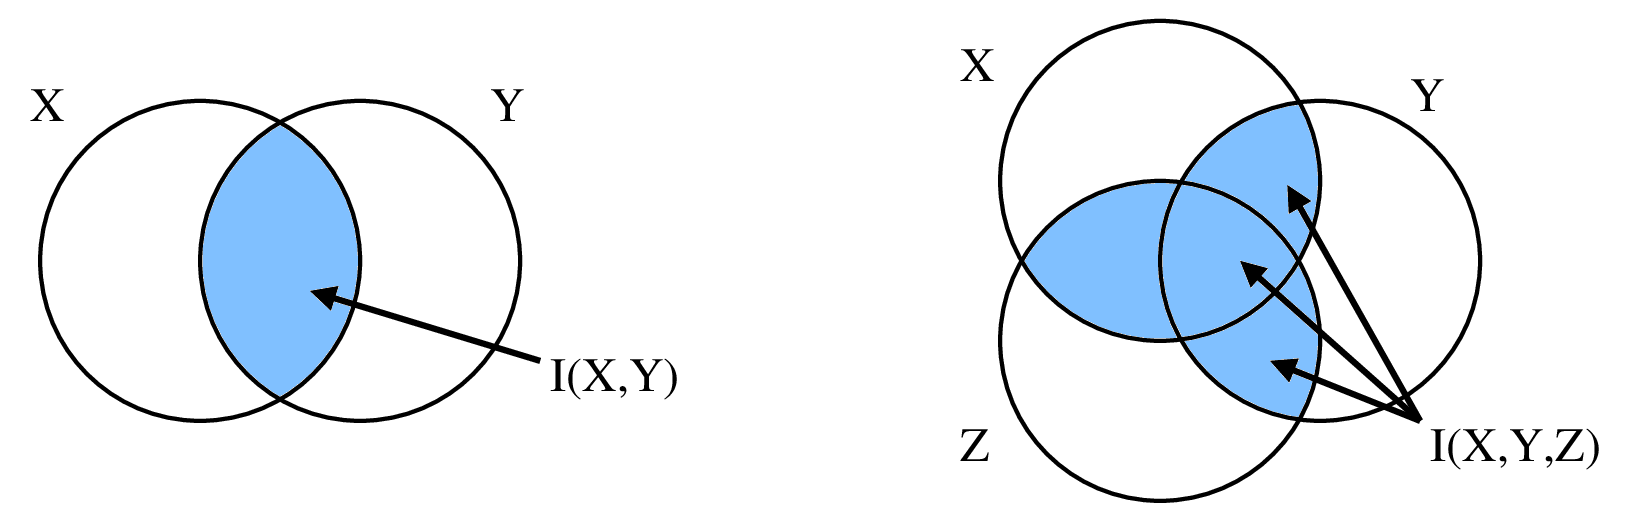
\includegraphics[height=1.5in]
{figs/mutual-information-edited.png}}
{Mutual information with two signals (left) and three signals (right).}
{fig-mutual-def}

% FIXME - Force a page break.
\clearpage
%
\section{Transfer Entropy}
\label{sect-entropy-transfer}

\textbf{Transfer entropy} can be thought of as the amount of information
about the future of variable Y that you learn by knowing the past of
variable X, in addition to what you already know from the past of variable
Y. This is illustrated in Figure \ref{fig-transfer-def-ce}. Transfer entropy
may be defined in terms of contitional entropy as shown in
Equation \ref{eq-transfer-def}:

\begin{equation}
TE_{X \rightarrow Y} = H(Y|Y_{past}) - H(Y|Y_{past},X_{past})
\label{eq-transfer-def}
\end{equation}

Transfer entropy may alternatively be defined in terms of conditional
mutual information, per Equation \ref{eq-transfer-def-mi}. This is
illustrated in Figure \ref{fig-transfer-def-mi}.

\begin{equation}
TE_{X \rightarrow Y} = I(X,X_{past}|Y_{past})
\label{eq-transfer-def-mi}
\end{equation}

The $Y_{past}$ and $X_{past}$ terms are usually approximated by taking the
past value at some time $t-\delta t$ as a proxy for the entire past history:

\begin{equation}
\begin{array}{cc}
\hat{Y}_{past} = Y(t - \delta t) \\
\hat{X}_{past} = X(t - \delta t) \\
\end{array}
\label{eq-transfer-past}
\end{equation}

\figdef{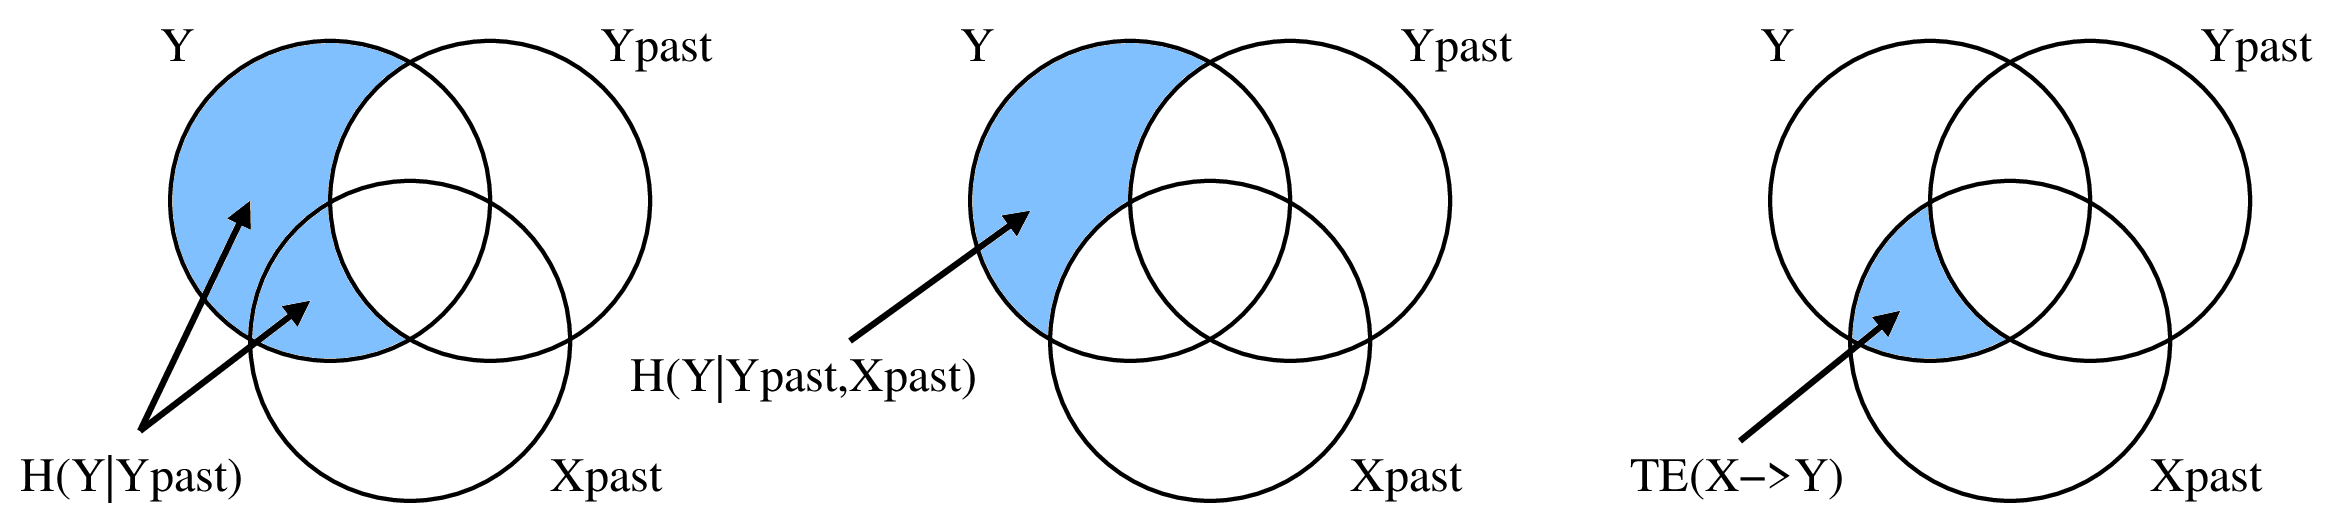
\includegraphics[height=1.5in]
{figs/transfer-entropy-ce-edited.png}}
{Transfer entropy between two signals, and its relation to conditional
entropy.}
{fig-transfer-def-ce}

\figdef{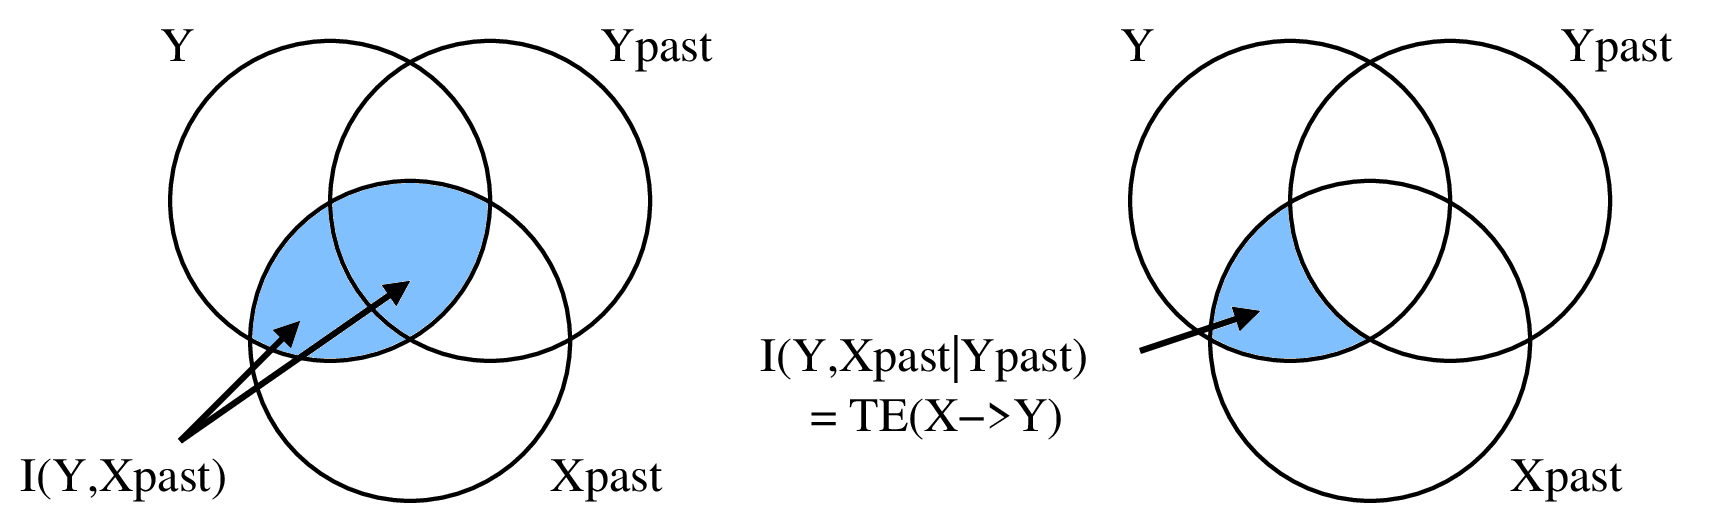
\includegraphics[height=1.5in]
{figs/transfer-entropy-mi-edited.png}}
{Transfer entropy between two signals, and its relation to mutual
information.}
{fig-transfer-def-mi}

% FIXME - Force a page break.
\clearpage
%
\textbf{Partial transfer entropy} is used to disentangle the contributions
of multiple variables to some Y variable. This is illustrated in
Figure \ref{fig-transfer-pte}. Partial transfer entropy is defined by
Equation \ref{eq-transfer-pte}:

\begin{equation}
pTE_{A \rightarrow Y} = H(Y|Y_{past},B_{past})
- H(Y|Y_{past},A_{past},B_{past})
\label{eq-transfer-pte}
\end{equation}

\figdef{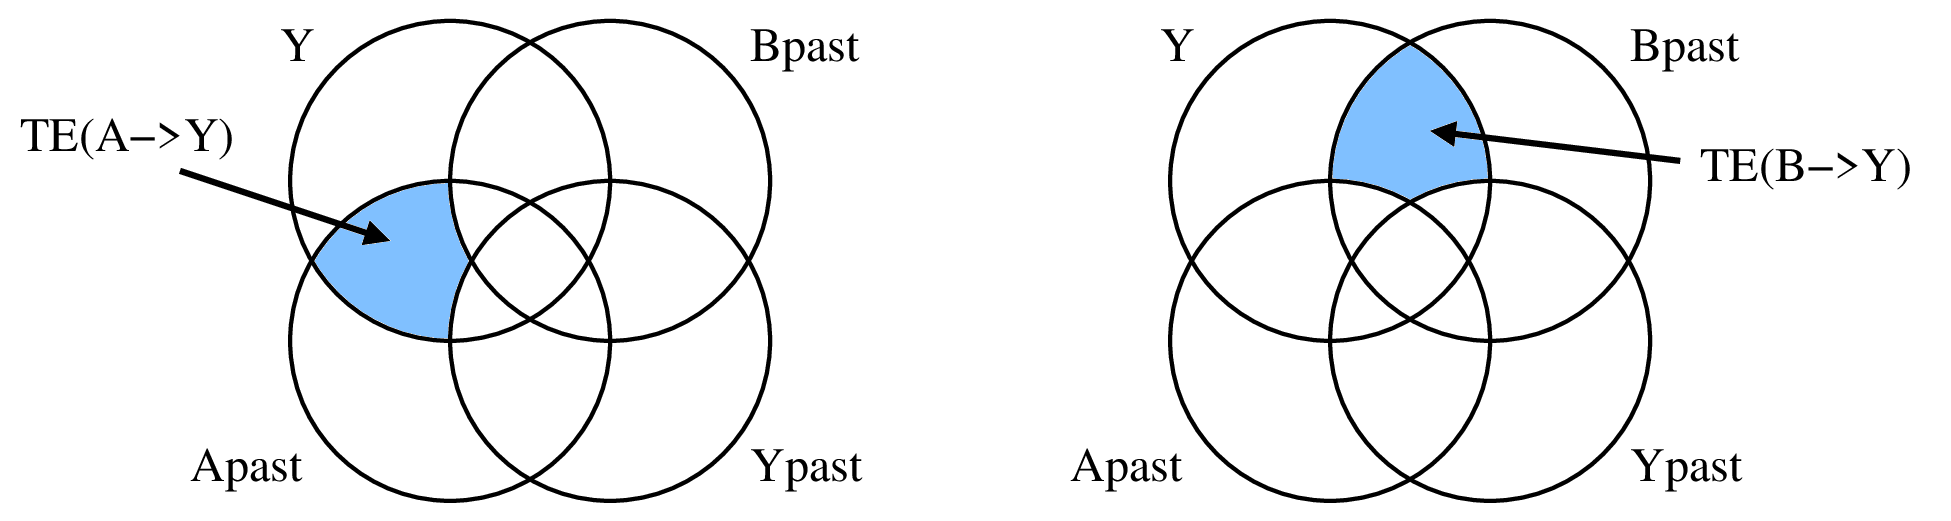
\includegraphics[height=1.5in]
{figs/transfer-entropy-pte-edited.png}}
{Partial transfer entropy between three signals.}
{fig-transfer-pte}

\section{References}
\label{sect-entropy-refs}

\begin{itemize}
%
\item C. E. Shannon, \textit{A Mathematical Theory of Communication},
The Bell System Technical Journal, v~27, pp~379--423,623-656, July, October,
1948
%
\end{itemize}

%
% This is the end of the file.
